%volby: 
% male × female
% czech × english (zatím funguje jen czech)
% a studijní program / obor 
% is_bc (nejvíc odladěno)
% api_bc
% api_ing
% edu_bc
% edu_ing

\documentclass[male,czech,api_bc]{kitheses}
\usepackage{ifthen}

\usepackage{amsmath,amssymb}
\usepackage{graphicx}
\usepackage{tikz}
\usetikzlibrary{shapes.geometric, shapes.symbols, positioning}
\usepackage{float}
\usepackage{color}
\usepackage{array}
\usepackage{longtable}
\usepackage{afterpage}
\usepackage{microtype}  % přesnější typografie

% workaround for imcompatibility of czech babel and biblatex

\iftutex
\else
\usepackage{etoolbox}
\makeatletter
\newcommand\my@hsyphen{-}
\newcommand\my@apostroph{'}
%%  \patchcmd\select@language{-}{\my@hyphen }{}{\fail}
% \patchcmd\select@language{'}{\my@apostroph }{}{\fail}
\makeatother
\fi

\usepackage[style=iso-numeric,shortnumeration=true]{biblatex}
\addbibresource{thesis.bib}


% fonty lze měnit (detaily viz sekce fonty)
\iftutex
	\usepackage{fontspec}  % nastavení fontů pro LuaLaTeX a XeLaTeX
%	\setmainfont{Libertinus Serif}
%	\setsansfont{Libertinus Sans}
%	\setmonofont[Scale=MatchLowercase]{Source Code Pro}
%	\usepackage{unicode-math}
%	\setmathfont{Libertinus Math}
\else
	\usepackage[utf8]{inputenc} % nastavení pro PDF LaTeX
	\usepackage[T1]{fontenc}
	\usepackage{libertinus}
	\renewcommand{\ttdefault}{pxtt}
\fi

\usepackage{csquotes} % uvozovky

% sazba ukázek kódu 

\usepackage{listings}

% ukázka pro nastavení balíku listings pro sazbu ukázek zdrojových kódů
\lstset{ %
  language=Python,                % the language of the code
  basicstyle=\small\ttfamily,    
  backgroundcolor=\color{white},   % choose the background color. You must add \usepackage{color}
  showspaces=false,                % show spaces adding particular underscores
  showstringspaces=true,           % underline spaces within strings
  showtabs=false,                  % show tabs within strings adding particular underscores
  frame=single,                    % adds a frame around the code
  tabsize=3,                       % sets default tabsize to 2 spaces
  breaklines=true,                 % sets automatic line breaking
  breakatwhitespace=false,         % sets if automatic breaks should only happen at whitespace
  keywordstyle=\color{blue}\bfseries,          % keyword style
  commentstyle=\color{darkgreen}\rmfamily,       % comment style
  stringstyle=\color{red}\itshape,         % string literal style
}

\lstdefinelanguage{Go}{
  keywords={break, default, func, interface, select, case, defer, go, map, struct, chan, else, goto, package, switch, const, fallthrough, if, range, type, continue, for, import, return, var},
  keywordstyle=\color{blue}\bfseries,
  ndkeywords={bool, int, int8, int16, int32, int64, uint, uint8, uint16, uint32, uint64, uintptr, float32, float64, complex64, complex128, byte, rune, string, error},
  ndkeywordstyle=\color{blue}\bfseries,
  sensitive=true,
  comment=[l]{//},
  morecomment=[s]{/*}{*/},
  commentstyle=\color{green}\rmfamily,
  stringstyle=\color{red}\itshape,
  morestring=[b]',
  morestring=[b]",
  morestring=[b]`
}

\lstdefinelanguage{CSharp}{
  keywords={abstract, as, base, bool, break, byte, case, catch, char, checked, class, const, continue, decimal, default, delegate, do, double, else, enum, event, explicit, extern, false, finally, fixed, float, for, foreach, goto, if, implicit, in, int, interface, internal, is, lock, long, namespace, new, null, object, operator, out, override, params, private, protected, public, readonly, ref, return, sbyte, sealed, short, sizeof, stackalloc, static, string, struct, switch, this, throw, true, try, typeof, uint, ulong, unchecked, unsafe, ushort, using, virtual, void, volatile, while, add, alias, ascending, async, await, by, descending, dynamic, equals, from, get, global, group, into, join, let, nameof, on, orderby, partial, remove, select, set, unmanaged, value, var, when, where, yield},
  keywordstyle=\color{blue}\bfseries,
  sensitive=true,
  comment=[l]{//},
  morecomment=[s]{/*}{*/},
  commentstyle=\color{green}\rmfamily,
  stringstyle=\color{red}\itshape,
  morestring=[b]',
  morestring=[b]"
}

\lstdefinelanguage{Gherkin}{
  keywords={Feature, Background, Scenario, Given, When, Then, And, But},
  keywordstyle=\color{blue}\bfseries,
  sensitive=true,
  comment=[l]{\#},
  commentstyle=\color{green}\rmfamily,
  stringstyle=\color{red}\itshape,
  morestring=[b]"
}

% barevné zvýraznění textů, které je nutno nahradit
\newcommand{\ZT}[1]{\colorbox{yellow}{\color{red}{#1}}}


% TOTO JE POTŘEBA ZMĚNIT !!!!!!
\newcommand{\nazevcz}{GoodAccess CLI klient pro Linux}        % zde VYPLŇTE český název práce (přesně podle zadání!)
\newcommand{\nazeven}{GoodAccess CLI client for Linux}     % zde VYPLŇTE anglický název práce (přesně podle zadání!)
\newcommand{\autor}{Valdemar Pospíšil}           % zde VYPLŇTE své jméno a příjmení
\newcommand{\rok}{\the\year}                
\newcommand{\vedouci}{Ing. Jiří Hromádka}         
% zde VYPLŇTE jméno a příjmení vedoucího práce, včetně titulů
\newcommand{\vedouciDAT}{Ing. Jiřímu Hromádkovi}   
% zde VYPLŇTE jméno a příjmení vedoucího práce, včetně titulů ve třetím pádě
                                                           

% zvětšuje o 23% vertikální okraje v tabulkách
\renewcommand{\arraystretch}{1.23}

% nastavení pro záhlaví (co nelze udělat v cls souboru)

\renewcommand{\chaptermark}[1]{\markboth{\arabic{chapter}. #1}{}}
\pagestyle{fancy}

% nastavení odkazů
\usepackage{url} % formátování URL, příkaz \url
\usepackage{varioref} % lepší interní odkazy na obrázky, apod. příkaz \vref
\usepackage[unicode=true,pdfusetitle,
 bookmarks=true,
 breaklinks=false,pdfborder={0 0 1},backref=false,colorlinks=false]{hyperref} % hypertextové odkazy v PDF
 
\newcommand{\UV}[1]{\quotedblbase#1\textquotedblleft}
 
% odstraňte pokud vám vadí absence zarovnání dole 
\raggedbottom

%%%%%%%%%%%%%%%%%%%%%%%%%%%%%%%%%%%%%%%%%%%%%%
% vlastní začátek dokumentu
%%%%%%%%%%%%%%%%%%%%%%%%%%%%%%%%%%%%%%%%%%%%%%

\begin{document}
\thispagestyle{empty}
\begin{center}
{
\LARGE
\univerzita\\[16pt]
\fakulta
}

\vspace{2cm}
\resizebox{8.42cm}{!}{%
\ifthenelse{\boolean{czech}}
{
\includegraphics{images/logos/LOGO_PRF_CZ_RGB_standard.jpg}}
{
\includegraphics{images/logos/LOGO_PRF_EN_RGB_standard.jpg}}}

\vspace{2cm}
{
\Huge\sffamily
\nazevcz\par
\vspace{0.6cm}
\Large\scshape \ifthenelse{\boolean{bc}}{bakalářská}{diplomová} práce
}
\end{center} 
 
\vfill
{
\large
\begin{tabular}{>{\bfseries}rl}
    Vypracoval: 	& \autor\\
    Vedoucí práce: 	& \vedouci\\
&\\
Studijní program:       & \program\\
\ifthenelse{\boolean{api}}{Studijní obor:          & \obor\\}{}
\end{tabular} 
}
\vspace{1.5cm}
\begin{center}
  \Large\scshape   Ústí nad Labem \rok
\end{center}

\cleardoublepage
\thispagestyle{empty}
\pagecolor{yellow}
{\Large Namísto žlutých stránek vložte digitálně podepsané zadání kvalifikační práce poskytnuté vedoucím katedry.\\\
Zadání musí zaujímat právě dvě strany.
}

Zadání je nutno vložit jako PDF pomocí některého nástroje, který umožňuje editaci dokumentů (se zachováním
elektronického podpisu).

V Linuxe lze například použít příkaz \texttt{pdftk}.

\clearpage
\thispagestyle{empty}
\afterpage{\nopagecolor}
~
\clearpage

\thispagestyle{empty} 
{\bfseries Prohlášení}

\vspace{0.5cm}
Prohlašuji, že jsem tuto \ifthenelse{\boolean{bc}}{bakalářskou}{diplomovou} práci vypracoval\ifthenelse{\boolean{feminum}}{a}{}
samostatně a použil\ifthenelse{\boolean{feminum}}{a}{}
jen pramenů, které cituji a uvádím v přiloženém seznamu literatury.

\vspace{0.5em}

Byl\ifthenelse{\boolean{feminum}}{a}{} jsem seznámen\ifthenelse{\boolean{feminum}}{a}{} 
s tím, že se na moji práci vztahují práva a povinnosti vyplývající ze
zákona č. 121/2000 Sb., ve znění zákona č. 81/2005 Sb., autorský zákon, zejména se
skutečností, že Univerzita Jana Evangelisty Purkyně v Ústí nad Labem má právo na uzavření
licenční smlouvy o užití této práce jako školního díla podle § 60 odst. 1 autorského zákona, a
s tím, že pokud dojde k užití této práce mnou nebo bude poskytnuta licence o užití jinému
subjektu, je Univerzita Jana Evangelisty Purkyně v Ústí nad Labem oprávněna ode mne
požadovat přiměřený příspěvek na úhradu nákladu, které na vytvoření díla vynaložila, a to
podle okolností až do jejich skutečné výše.

\vspace{2em}

V Ústí nad Labem dne \today   \hfill Podpis: \makebox[4cm][s]{\dotfill}

\cleardoublepage
\thispagestyle{empty}
~
\vfill

\begin{flushright}
    Děkuji vedoucímu práce \ZT{\vedouciDAT}\\ 
    za neocenitelné rady a pomoc při tvorbě bakalářské práce.
\end{flushright}

\cleardoublepage

\textsc{\nazevcz}

\textbf{Abstrakt:}

V současné době nabízí GoodAccess VPN řešení především prostřednictvím grafického uživatelského rozhraní, což nevyhovuje všem uživatelským scénářům. Zejména v prostředí serverů, automatizovaných systémů a DevOps pracovních postupů preferují administrátoři a pokročilí uživatelé řešení příkazové řádky.

Hlavním cílem této práce je navrhnout a implementovat funkční prototyp CLI aplikace pro správu GoodAccess VPN připojení na Linux distribucích s využitím WireGuard protokolu. Práce se zabývá návrhem architektury, bezpečným ukládáním dat a implementací komunikace se systémovou službou pomocí IPC.

\textbf{Klíčová slova:} VPN, GoodAccess, CLI, Linux, Go, .NET, WireGuard, IPC, Clean Architecture

\bigskip


\textsc{\nazeven}

\textbf{Abstract:}

Currently, GoodAccess VPN offers solutions primarily through a graphical user interface, which does not suit all user scenarios. Especially in server environments, automated systems, and DevOps workflows, administrators and advanced users prefer command-line solutions.

The main goal of this work is to design and implement a functional prototype of a CLI application for managing GoodAccess VPN connections on Linux distributions using the WireGuard protocol. The work deals with the design of the architecture, secure data storage, and implementation of communication with the system service using IPC.

\textbf{Keywords:} VPN, GoodAccess, CLI, Go, .NET, WireGuard

\tableofcontents

\cleardoublepage
\section*{Seznam použitých zkratek}
\begin{description}
    \item[API] Application Programming Interface
    \item[APT] Advanced Package Tool
    \item[BDD] Behavior-Driven Development
    \item[CI] Continuous Integration
    \item[CLI] Command Line Interface
    \item[DAC] Discretionary Access Control
    \item[E2E] End-to-End
    \item[FHS] Filesystem Hierarchy Standard
    \item[GUI] Graphical User Interface
    \item[IPC] Inter-Process Communication
    \item[JSON] JavaScript Object Notation
    \item[OIDC] OpenID Connect
    \item[PID] Process Identifier
    \item[POSIX] Portable Operating System Interface
    \item[QA] Quality Assurance
    \item[SDLC] Software Development Life Cycle
    \item[SDP] Software Defined Perimeter
    \item[SSH] Secure Shell
    \item[SSO] Single Sign-On
    \item[TDD] Test-Driven Development
    \item[TUI] Text User Interface
    \item[UDS] Unix Domain Sockets
    \item[UID] User Identifier
    \item[VPN] Virtual Private Network
    \item[XP] Extreme Programming
    \item[ZTNA] Zero Trust Network Access
\end{description}

% ============================================================================
% ZDE ZAČÍNÁ VKLÁDÁNÍ TVÝCH KAPITOL
% ============================================================================

% Úvod (musí obsahovat \addchap{Úvod})
\addchap{Úvod}
\label{chap:uvod}

V posledních letech došlo k zásadnímu posunu v organizaci práce a správě síťové infrastruktury. S masivním přechodem na práci na dálku a distribuované týmy se tradiční modely zabezpečení sítě ukazují jako nedostatečné. Organizace stále častěji adoptují architektury typu Zero Trust Network Access (ZTNA), kde je bezpečné VPN připojení klíčovým prvkem nejen pro koncové uživatele, ale i pro serverovou infrastrukturu.

Platforma GoodAccess v současné době nabízí řešení primárně prostřednictvím grafického uživatelského rozhraní (GUI). Toto řešení je vhodné pro běžné uživatele na osobních počítačích, avšak naráží na limity v prostředí serverů, automatizovaných systémů a DevOps pracovních postupů.

V serverovém prostředí Linux, které je dominantní platformou pro cloudovou infrastrukturu, často není grafické rozhraní dostupné (tzv. headless servery). Administrátoři a DevOps inženýři vyžadují nástroje, které lze ovládat z příkazové řádky, snadno skriptovat a integrovat do CI/CD pipelin. Absence nativního CLI (Command Line Interface) klienta pro Linux představuje pro GoodAccess značné omezení v možnosti nasazení v těchto scénářích.


% Teorie (musí obsahovat \chapter{Teoretická východiska} atd.)
\chapter{Teoretická východiska}
\label{chap:teorie}

Tato kapitola analyzuje klíčové technologie, architektonické principy a bezpečnostní standardy nezbytné pro návrh moderního CLI nástroje v prostředí OS Linux. Text postupuje od obecné problematiky příkazové řádky přes síťové protokoly až po specifika implementačních platforem .NET a Go.

\section{Rozhraní příkazové řádky}
\label{sec:cli_teorie}
Rozhraní příkazové řádky (CLI – Command Line Interface) představuje jeden z nejstarších, avšak stále nejvýkonnějších způsobů interakce uživatele s počítačem. Navzdory masivnímu rozšíření grafických uživatelských rozhraní (GUI) v 90. letech 20. století zůstává CLI nepostradatelným nástrojem pro systémové administrátory, vývojáře a pokročilé uživatele, zejména v prostředí operačních systémů typu Unix a Linux.

\subsection{Role CLI v moderní správě systémů}
Hlavním důvodem preference příkazové řádky v profesionálním prostředí je efektivita, rychlost a snadná automatizace. Zatímco grafické rozhraní je navrženo pro intuitivní objevování funkcí pomocí vizuálních prvků, CLI se zaměřuje na precizní a opakovatelné provádění úkolů. Administrátor může pomocí jediného příkazu nebo krátkého skriptu provést operaci na stovkách serverů současně, což je v rámci GUI prakticky neproveditelné.

Dalším kritickým faktorem je vzdálená správa. Protokol SSH (Secure Shell), který je de facto standardem pro správu linuxových serverů, je primárně textově orientovaný. Přenos textových příkazů a jejich výstupů vyžaduje minimální síťovou propustnost, což umožňuje spolehlivou správu systémů i přes nestabilní nebo pomalé připojení. V prostředí cloudu a kontejnerizace (např. Docker, Kubernetes), kde systémy často nemají žádné grafické výstupní zařízení (headless režim), je CLI jedinou možností interakce.

\subsection{Principy návrhu a standardy CLI aplikací}
Kvalitní CLI aplikace se řídí souborem ustálených principů, které zajišťují jejich předvídatelnost a vzájemnou spolupráci. Eric S. Raymond ve své knize \textit{The Art of Unix Programming} definuje tzv. „Unixovou filosofii“, jejímž základem je tvorba malých, jednoúčelových nástrojů, které spolu efektivně komunikují \cite{raymond_unix}. Tento přístup umožňuje skládat komplexní operace z jednoduchých komponent pomocí mechanismu rour (pipes).

Základním stavebním kamenem interakce v CLI jsou standardní datové proudy:
\begin{itemize}
    \item \textbf{Standardní vstup (stdin):} Zdroj dat pro aplikaci, typicky klávesnice nebo výstup jiného programu.
    \item \textbf{Standardní výstup (stdout):} Primární kanál pro výstup dat, typicky terminál.
    \item \textbf{Standardní chybový výstup (stderr):} Oddělený kanál pro chybová hlášení a diagnostiku, což umožňuje uživateli přesměrovat data do souboru, zatímco chyby stále vidí na obrazovce.
\end{itemize}

Důležitou roli hraje také syntaxe příkazů. Moderní nástroje se snaží dodržovat standardy jako POSIX nebo GNU konvence pro argumenty a přepínače (flags). Krátké přepínače (např. \texttt{-v}) jsou určeny pro rychlé psaní, zatímco dlouhé varianty (např. \texttt{--verbose}) zvyšují čitelnost skriptů a dokumentace.

\subsection{CLI versus TUI}
V rámci terminálu se můžeme setkat také s textovým uživatelským rozhraním (TUI – Text User Interface). Na rozdíl od klasického CLI, které vypisuje řádky textu v sekvenčním pořadí, TUI využívá celou plochu terminálu k vykreslování vizuálních prvků, jako jsou okna, menu, tabulky nebo interaktivní grafy, často s využitím knihoven jako \texttt{ncurses} nebo moderních frameworků v jazyce Go (např. \texttt{Bubble Tea}).

Hlavní rozdíl spočívá v komplexitě a způsobu interakce. CLI je ideální pro jednorázové příkazy a automatizaci v nekonečném proudu (batch processing). TUI je naproti tomu vhodnější pro interaktivní nástroje, kde uživatel potřebuje neustálý přehled o stavu systému nebo kde je navigace v datech pomocí klávesových zkratek efektivnější než vypisování parametrů (např. textové editory, správci souborů nebo dashboardy pro monitoring).

\section{Architektura VPN a principy Zero Trust}
\label{sec:vpn_zero_trust}
Tradiční pojetí zabezpečení sítě, založené na ochraně perimetru, prochází v posledních letech zásadní transformací. Tato sekce popisuje evoluci od klasických VPN tunelů k moderní architektuře Zero Trust Network Access (ZTNA).

\subsection{Tradiční VPN a perimetrová bezpečnost}
Virtuální privátní síť (VPN) je technologie, která umožňuje vytvořit bezpečné, šifrované spojení (tunel) mezi dvěma body v rámci nezabezpečené sítě, jako je internet. Princip tunelování spočívá v zapouzdření (enkapsulaci) síťových paketů do jiného protokolu, který zajišťuje integritu a důvěrnost přenášených dat.

Historicky se organizace spoléhaly na model „hrad a příkop“ (Castle-and-Moat). V tomto modelu je vnitřní síť považována za důvěryhodnou zónu, která je od vnějšího světa oddělena firewallem (příkopem). VPN v tomto kontextu slouží jako „padací most“, který umožňuje vzdáleným uživatelům vstoupit do vnitřní sítě. Jakmile však uživatel získá přístup, má často široký dosah k mnoha zdrojům v rámci sítě. Tento přístup trpí kritickou slabinou: pokud útočník kompromituje jediné zařízení uvnitř perimetru, může se v síti volně pohybovat (laterální pohyb) a napadat další systémy, protože vnitřní síť mu implicitně důvěřuje.

\subsection{Zero Trust Network Access (ZTNA) a GoodAccess}
Filozofie Zero Trust (nulová důvěra) tento model opouští a vychází z principu „nikdy nedůvěřuj, vždy prověřuj“ (Never trust, always verify). V architektuře ZTNA není důvěra nikdy udělena na základě fyzického umístění uživatele nebo jeho IP adresy. Každý pokus o přístup k jakémukoliv zdroji musí být individuálně autentizován, autorizován a šifrován.

Klíčovým prvkem ZTNA je Software Defined Perimeter (SDP). SDP vytváří dynamickou, virtuální hranici kolem aplikací a služeb, čímž je činí „neviditelnými“ pro veřejný internet i pro neautorizované uživatele v lokální síti. GoodAccess implementuje tyto principy formou cloudové platformy, která nahrazuje tradiční VPN brány \cite{goodaccess_doc}. Místo statických IP adres využívá identitu uživatele (často propojenou s SSO/OIDC) a kontext zařízení (tzv. Device Posture) k dynamickému přidělování přístupových práv k jednotlivým systémům \cite{goodaccess_architecture}. Tím se radikálně snižuje plocha možného útoku, protože uživatel vidí pouze ty zdroje, ke kterým má explicitní oprávnění.

\subsection{Srovnání protokolů WireGuard a OpenVPN}
Pro realizaci samotného šifrovaného spojení na platformě Linux využívá GoodAccess dva dominantní protokoly: OpenVPN a WireGuard. Každý z nich představuje jinou generaci technologií a liší se především architekturou a flexibilitou správy.

OpenVPN je dlouholetým standardem v oblasti VPN. Je postaven na knihovně OpenSSL a nabízí extrémně široké možnosti konfigurace, včetně podpory různých šifrovacích algoritmů a transportních protokolů (UDP i TCP). Tato univerzalita je však vykoupena vysokou komplexitou zdrojového kódu (stovky tisíc řádků), což ztěžuje bezpečnostní audity a vede k vyšší režii při zpracování paketů, zejména v uživatelském prostoru.

Naproti tomu WireGuard je moderní protokol navržený s důrazem na jednoduchost, rychlost a moderní kryptografii \cite{wireguard_paper}. S rozsahem přibližně 4 000 řádků kódu je WireGuard snadno auditovatelný a díky implementaci přímo v jádře Linuxu dosahuje výrazně vyšší propustnosti a nižší latence než OpenVPN. Z pohledu správy systému se WireGuard chová jako standardní síťové rozhraní, což zjednodušuje konfiguraci směrování a integraci do systémových nástrojů. Pro dynamické enterprise prostředí, které GoodAccess obsluhuje, je WireGuard ideální volbou díky rychlému navazování spojení (handshake) a vysoké odolnosti vůči změnám síťového prostředí.

\section{Architektura OS Linux a správa systému}
\label{sec:linux_architektura}
Pro pochopení interakce mezi CLI klientem a systémovými prostředky je nutné definovat hranice mezi uživatelským prostorem a jádrem.

\subsection{Jádro, Netlink a virtuální FS}
Operační systém Linux striktně odděluje privilegovaný prostor jádra (Kernel Space) od uživatelského prostoru (User Space). Pro aplikace typu VPN klienta je klíčová schopnost konfigurovat síťové parametry, které spravuje právě jádro. K tomuto účelu Linux poskytuje několik rozhraní.

Virtuální souborové systémy \texttt{/proc} a \texttt{/sys} umožňují aplikacím číst stav systému a měnit některé parametry pouhým zápisem do souboru (např. povolení IP forwardingu). Nicméně pro komplexnější operace, jako je vytváření síťových rozhraní nebo správa směrovacích tabulek, se využívá rozhraní \texttt{Netlink}. Jak uvádí Ward \cite{ward_linux}, \texttt{Netlink} je socketové rozhraní sloužící ke komunikaci mezi jádrem a uživatelskými procesy. V této práci je \texttt{Netlink} využíván nepřímo skrze systémové nástroje nebo knihovny v .NET, které zajišťují nízkoúrovňovou konfiguraci WireGuard rozhraní.

\subsection{Správa služeb a Systemd}
Moderní linuxové distribuce využívají jako inicializační systém a správce služeb \texttt{systemd}. Pro aplikaci GoodAccess CLI je \texttt{systemd} zásadní, protože zajižduje běh backendové služby (\texttt{CLIService}) jako systémového démona, který je spouštěn při startu systému a automaticky restartován v případě chyby. \texttt{systemd} také umožňuje definovat závislosti služeb, což zaručuje, že se VPN služba pokusí o navázání spojení až ve chvíli, kdy je dostupné síťové rozhraní. V rámci této práce jsou vytvořeny \textit{unit} soubory, které definují životní cyklus služby a její integraci do systému.

\subsection{Bezpečné ukládání tajemství (Secure Storage)}
Kritickým aspektem VPN klienta je ochrana privátních klíčů a tokenů. Linux standardně využívá \textit{Secret Service API} komunikující přes DBus, což umožňuje aplikacím ukládat tajemství do klíčenky (Keyring) spravované systémem, nikoliv do prostých textových souborů.

\section{Implementační technologie}
\label{sec:technologie}
Architektura řešení je rozdělena na privilegovanou službu (Daemon) a uživatelské rozhraní (Client).

\subsection{Backend: Platforma .NET}
Pro implementaci systémové služby (Daemon) byla zvolena platforma .NET 8. Tato volba vychází především z potřeby kontinuity s existující infrastrukturou GoodAccess, která je na technologiích Microsoft .NET postavena. .NET na Linuxu dnes nabízí vysoký výkon a plnou podporu pro systémové programování, včetně nativní interakce s nízkoúrovňovými API systému přes P/Invoke nebo knihovny typu Microsoft.Extensions.Hosting pro běh služeb. Modul \texttt{CLIService} tak může sdílet klíčovou logiku pro správu tokenů, certifikátů a stavu tunelu se stávajícím grafickým klientem, což zaručuje konzistentní chování aplikace napříč různými rozhraními.

\subsection{Frontend: Jazyk Go a TUI}
Pro klientskou část (CLI frontend) byl zvolen jazyk Go. Go se v posledních letech stal de facto standardem pro vývoj cloud-native a systémových nástrojů v ekosystému Linux (např. Docker, Kubernetes, Terraform). Hlavní výhodou je schopnost kompilace do jediné staticky linkované binárky bez nutnosti instalace runtime prostředí, což je pro nástroj příkazové řádky ideální. Go nabízí vynikající knihovny pro tvorbu moderních terminálových rozhraní – v této práci je využita knihovna \texttt{Cobra} pro definici struktury příkazů a framework \texttt{Bubble Tea} pro reaktivní zobrazení stavu a interaktivní prvky.

\subsection{Meziprocesová komunikace (IPC)}
V architektuře, kde je logika aplikace oddělena od uživatelského rozhraní do samostatných procesů, hraje klíčovou roli meziprocesová komunikace (IPC – Inter-Process Communication). Pro potřeby této práce byla zvolena technologie Unix Domain Sockets (UDS).

Unix Domain Sockets představují datový komunikační koncový bod pro výměnu dat mezi procesy běžícími na stejném hostitelském operačním systému. Na rozdíl od síťových socketů (TCP/IP), které jsou určeny pro komunikaci přes síť, UDS nevyužívají síťový zásobník (network stack), což výrazně snižuje režii a zvyšuje propustnost komunikace.

Z pohledu bezpečnosti, která je u VPN klienta kritická, nabízejí UDS zásadní výhodu v podobě využití standardních souborových oprávnění systému Linux. Přístup k socketu lze omezit na konkrétního uživatele nebo skupinu, čímž se zamezí neoprávněným aplikacím v komunikaci se systémovou službou. V navržené architektuře slouží UDS jako transportní vrstva pro protokol gRPC, který zajišťuje silně typované rozhraní pro příkazy jako autentizace, připojení nebo monitoring stavu.

\section{Distribuce softwaru}
\label{sec:distribuce}
Zadání práce vyžaduje přípravu balíčků pro distribuce Debian a Fedora.
% Zde popiš .deb a .rpm formáty

\section{Metodika vývoje}
\label{sec:metodika}
% Zde použij svůj text o XP a Beckovi


% Analýza
\chapter{Analýza a specifikace požadavků}
\label{chap:analyza}

Celý proces analýzy a sběru požadavků probíhal v agilním prostředí. Během vývoje se využívaly iterativní schůzky, pravidelné standupy a dedikované brainstormové sekce. Na těchto setkáních byli přítomni zkušení vývojáři a technický ředitel (CTO), který díky přímému kontaktu se zákazníky detailně znal jejich konkrétní požadavky a tlumočil jejich zpětnou vazbu. Díky tomu bylo možné rychle a efektivně reagovat na potřeby uživatelů a správně specifikovat klíčové vlastnosti aplikace.

\section{Identifikace zúčastněných stran}
Primárními uživateli GoodAccess CLI pro Linux jsou:
\begin{itemize}
    \item \textbf{System Administrators:} Spravují servery a vyžadují stabilní nástroj pro vzdálenou správu přes SSH bez nutnosti grafického rozhraní.
    \item \textbf{DevOps Inženýři:} Potřebují integrovat VPN připojení do automatizovaných skriptů a CI/CD pipelines. Vyžadují predikovatelné chování a strojově čitelný výstup.
    \item \textbf{Běžní zaměstnanci:} Uživatelé, kteří preferují textové uživatelské rozhraní (TUI) před grafickým klientem (GUI) pro každodenní práci.
\end{itemize}

\section{Případy užití}
Hlavní scénáře použití systému z pohledu koncového uživatele (administrátora či běžného zaměstnance) ukazuje následující diagram případů užití (Obrázek \ref{fig:usecase}).

\begin{figure}[H]
    \centering
    \begin{tikzpicture}[scale=1.0, transform shape, font=\sffamily,
        usecase/.style={rectangle, rounded corners=3ex, draw=black, fill=blue!5, text centered, inner sep=2mm, text width=3.5cm, minimum height=1cm},
        actor/.style={draw=none, fill=none, text centered},
        line/.style={-, thick, draw=black!70}]

        % Hranice systému
        \draw[thick, draw=black!50, rounded corners=1ex, fill=gray!5] (-0.5, -4.5) rectangle (4.5, 5.5);
        \node at (2, 5) {\large \textbf{GoodAccess CLI}};

        % Uživatel (stickman)
        \node[actor] (user) at (-3.5, 0.5) {
            \begin{tikzpicture}[scale=0.8]
                \draw[thick] (0,0.5) circle (0.3); % Hlava
                \draw[thick] (0,0.2) -- (0,-0.6); % Tělo
                \draw[thick] (-0.4,-0.1) -- (0.4,-0.1); % Ruce
                \draw[thick] (0,-0.6) -- (-0.4,-1.2); % Levá noha
                \draw[thick] (0,-0.6) -- (0.4,-1.2); % Pravá noha
                \node at (0,-1.6) {\textbf{Uživatel}};
            \end{tikzpicture}
        };

        % Use Cases
        \node[usecase] (setup) at (2, 4) {Prvotní nastavení\\(Setup)};
        \node[usecase] (login) at (2, 2.5) {Přihlášení\\(Login)};
        \node[usecase] (connect) at (2, 1) {Připojení k VPN\\(Connect)};
        \node[usecase] (status) at (2, -0.5) {Zjištění stavu\\(Status)};
        \node[usecase] (disconnect) at (2, -2) {Odpojení VPN\\(Disconnect)};
        \node[usecase] (logout) at (2, -3.5) {Odhlášení\\(Logout)};

        % Vztahy
        \draw[line] (user) -- (setup.west);
        \draw[line] (user) -- (login.west);
        \draw[line] (user) -- (connect.west);
        \draw[line] (user) -- (status.west);
        \draw[line] (user) -- (disconnect.west);
        \draw[line] (user) -- (logout.west);
    \end{tikzpicture}
    \caption{Diagram případů užití GoodAccess CLI}
    \label{fig:usecase}
\end{figure}

\section{Funkční požadavky}
\label{sec:funkcni_pozadavky}
Na základě analýzy potřeb byly stanoveny následující funkční požadavky:

\subsection{Autentizace a správa relace}
Aplikace musí umožnit přihlášení uživatele v prostředí bez webového prohlížeče. Z tohoto důvodu nepodporuje přihlášení pomocí webového SSO (Single Sign-On).
\begin{itemize}
    \item \textbf{F1 -- Login:} Přihlášení probíhá pomocí standardního terminálového vstupu, kam uživatel zadá název týmu, uživatelské jméno a heslo. Zadávání hesla je pro bezpečnost maskováno (zobrazují se pouze znaky \texttt{*}).
    \item \textbf{F2 -- Logout:} Standardní ukončení relace uživatele a bezpečné smazání lokálně uložených tokenů.
    \item \textbf{F3 -- Setup:} Interaktivní průvodce prvotním nastavením (onboarding wizard). Umožňuje uživateli v jednom kroku provést přihlášení, zvolit protokol, vybrat bránu, nastavit perzistentní připojení a rovnou se připojit. Tento proces je striktně interaktivní.
\end{itemize}

\subsection{Správa připojení}
Jádrem aplikace je ovládání VPN tunelu a správa nastavení pro připojení.
\begin{itemize}
    \item \textbf{F4 -- Connect:} Navázání připojení. Standardně se využije preferovaný protokol a brána (gateway) uložená z předchozího nastavení.
    \item \textbf{F5 -- Connect Flags:} Možnost dočasně přepsat preferované nastavení při připojení pomocí přepínačů \texttt{-g} (gateway) a \texttt{-p} (protocol). Přepínač \texttt{--protocol} očekává textový název protokolu, zatímco \texttt{--gateway} vyvolá interaktivní výběr. Tato volba se neuloží jako preferovaná.
    \item \textbf{F6 -- Disconnect:} Korektní ukončení VPN připojení a úklid routovacích pravidel.
    \item \textbf{F7 -- Persistent Connect:} Nastavení připojení na úrovni celého zařízení, které zajistí automatické znovupřipojení i po restartu počítače.
    \item \textbf{F8 -- Gateway Selection:} Možnost uživatele vybrat si konkrétní VPN bránu.
    \item \textbf{F9 -- Protocol Selection:} Možnost uživatele zvolit preferovaný VPN protokol (WireGuard nebo OpenVPN).
\end{itemize}

\subsection{Monitoring a stav}
\begin{itemize}
    \item \textbf{F10 -- Status:} Zobrazení aktuálního stavu připojení (Připojeno/Odpojeno, IP adresa, přenesená data). Výstup lze volitelně formátovat do JSON pro snadné strojové zpracování.
\end{itemize}

\subsection{Obecné příkazy}
\begin{itemize}
    \item \textbf{F11 -- Version:} Zobrazení aktuální verze aplikace.
    \item \textbf{F12 -- Help:} Zobrazení standardní nápovědy k dostupným příkazům a jejich použití.
\end{itemize}

\section{Mimofunkční požadavky}
\label{sec:nefunkcni_pozadavky}
\begin{itemize}
    \item \textbf{M1 -- Výkon a odezva:} Aplikace v prostředí příkazové řádky (CLI) musí reagovat okamžitě. Zásadní je rychlý start aplikace a nízká paměťová náročnost, aby její spuštění uživatele neomezovalo.
    \item \textbf{M2 -- Kompatibilita:} Aplikace musí být funkční na hlavních serverových distribucích Linuxu (Debian/Ubuntu, Fedora/RHEL).
    \item \textbf{M3 -- Bezpečnost:} Citlivá data (přístupové tokeny, privátní klíče) musí být uložena bezpečně a přístupná pouze oprávněné službě.
    \item \textbf{M4 -- Distribuce a nasazení:} Pro usnadnění instalace a správy ze strany systémových administrátorů musí být aplikace zabalitelná do standardních distribučních balíčků. Konkrétně se jedná o formáty \texttt{.deb} (pro rodinu Debian) a \texttt{.rpm} (pro rodinu Red Hat).
\end{itemize}

\section{Analýza architektury}
\label{sec:analyza_architektury}
\subsection{Analýza stávajícího řešení GoodAccess}
Aplikace GoodAccess na operačním systému Linux v současné době funguje jako rozdělený systém složený ze dvou hlavních komponent:

\begin{itemize}
    \item \textbf{GoodAccessService (Daemon):} Tato služba běží na pozadí pod správou systému \texttt{systemd} s právy uživatele \texttt{root}. Její primární odpovědností je správa síťových rozhraní (především tunelů WireGuard), konfigurace systémového směrování (routingu) a bezpečné uchovávání kryptografických klíčů a certifikátů.
    \item \textbf{Grafický klient (Electron/GUI):} Uživatelské rozhraní je postaveno na frameworku Electron. Tato část běží v běžném uživatelském prostoru (bez root oprávnění) a funguje v podstatě jako „hloupý“ prezentační ovladač. Zobrazuje stav a přijímá příkazy od uživatele, které následně předává daemonu ke zpracování. Komunikace mezi těmito dvěma procesy probíhá lokálně, typicky pomocí Unix Domain Sockets (IPC).
\end{itemize}

\subsection{Možné architektonické přístupy}
Při návrhu řešení byly zvažovány dva přístupy k interakci s existující logikou GoodAccess:

\begin{description}
    \item[Návrh A: Tenký klient (Wrapper)] V tomto modelu běží v systému jedna privilegovaná služba (.NET), která drží stav a vykonává operace. CLI aplikace (Go) slouží pouze jako dálkové ovládání, které posílá příkazy službě přes IPC.
    \item[Návrh B: Samostatná logika] CLI aplikace by obsahovala veškerou logiku pro připojení a správu WireGuardu a běžela by přímo pod uživatelem \texttt{root}, nezávisle na existující službě.
\end{description}

\subsection{Zvolené řešení}
Byl zvolen \textbf{Návrh A (Wrapper)} z následujících důvodů:
\begin{enumerate}
    \item \textbf{Single Source of Truth:} Služba drží jednotný stav aplikace. Nedochází k desynchronizaci mezi tím, co si myslí CLI, a tím, co je reálně nastaveno v síti.
    \item \textbf{Bezpečnost:} Uživatel nemusí spouštět CLI pod \texttt{rootem}. Privilegované operace provádí pouze izolovaná služba na pozadí.
    \item \textbf{Znovupoužitelnost:} Využívá se již otestovaná a existující logika v .NET backendu, což je v souladu s hodnotou jednoduchosti (Simplicity) metodiky Extreme Programming (\ref{sec:agile_teorie}).
\end{enumerate}

%\begin{figure}[H]
%    \centering
%    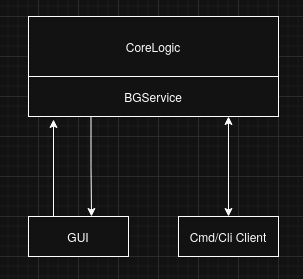
\includegraphics[width=0.8\textwidth]{images/architecture.png}
%    \caption{Zvolená architektura: Tenký klient (Wrapper)}
%    \label{fig:architecture}
%\end{figure}


% Návrh
\chapter{Návrh řešení}
\label{chap:navrh}

V této kapitole je představen detailní technický návrh prototypu CLI klienta a navazující síťové služby. Návrh přímo vychází ze zvolené architektury tenkého klienta, která byla zdůvodněna v předchozí kapitole (viz sekce \ref{sec:analyza_architektury}).

\section{Komponenty systému}
Celý systém je v souladu se zvoleným návrhem rozdělen na dvě hlavní, technologicky odlišné komponenty, které spolu komunikují přes definované rozhraní.

\begin{itemize}
    \item \textbf{Služba (Service - .NET):} Funguje jako daemon spravovaný systémem \texttt{systemd} s právy uživatele \texttt{root}. Její primární a jedinou odpovědností je správa stavu sítě, konfigurace rozhraní WireGuard a bezpečné ukládání kryptografických klíčů. Volba platformy .NET pro tuto komponentu přímo vychází z potřeby multiplatformní podpory a snadné integrace do systému \texttt{systemd} (viz sekce \ref{sec:technologie}), a především umožňuje znovupoužití již existující a otestované logiky z grafického klienta (viz sekce \ref{sec:analyza_architektury}).
    \item \textbf{Klient (Client - Go):} Běží v uživatelském prostoru (bez \texttt{root} oprávnění) a zajišťuje čistě interakci s uživatelem. Zodpovídá za parsování argumentů příkazové řádky pomocí frameworku \texttt{Cobra}, obsluhu interaktivních TUI prvků prostřednictvím \texttt{Bubble Tea} a finální formátování výstupu. Jazyk Go byl pro vývoj CLI zvolen díky svým vlastnostem pro systémové programování, rychlému startu a statické kompilaci do jediné binárky, což radikálně zjednodušuje distribuci (viz sekce \ref{sec:technologie} a \ref{sec:cli_teorie}).
\end{itemize}

Architektura Go klienta navíc úzce reflektuje principy takzvané \textit{Clean Architecture}. Celá kódová základna klienta je rozdělena do logických vrstev, kde uživatelské rozhraní (UI a parsování příkazů) je zcela odděleno od aplikační logiky a transportní vrstvy (IPC komunikace přes Unix Domain Sockets). Toto vrstvení zaručuje vysokou testovatelnost komponent a možnost nezávisle upravovat vizuální prezentaci bez vlivu na způsob, jakým klient komunikuje s .NET službou.

\begin{figure}[H]
    \centering
    % TODO: Přidat skutečný obrázek architektury
    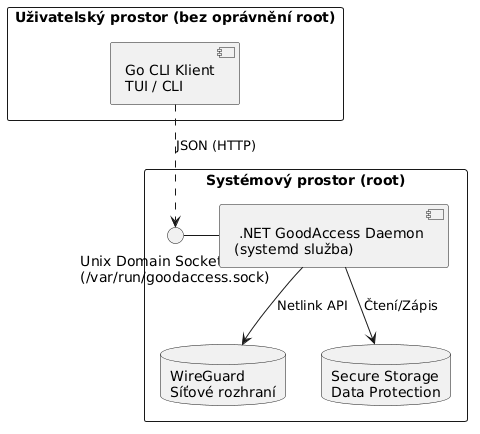
\includegraphics[width=0.8\textwidth]{images/navrh-architecture.png}
    \caption{Architektura systému znázorňující hranici mezi .NET Službou a Go Klientem skrze IPC (Unix Domain Sockets).}
    \label{fig:architecture_ipc}
\end{figure}

\begin{figure}[H]
    \centering
    % TODO: Přidat skutečný obrázek Clean Architecture
    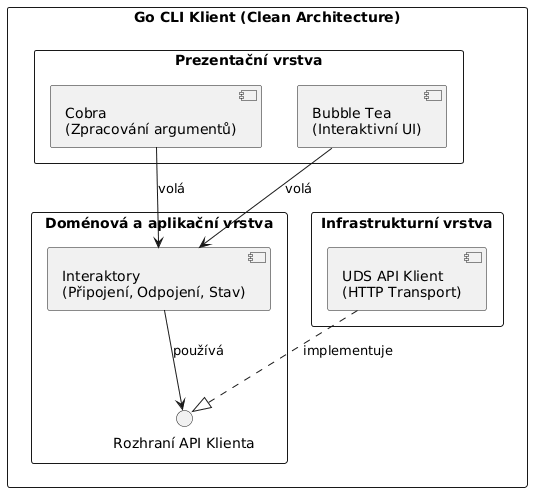
\includegraphics[width=0.8\textwidth]{images/clean-architecture.png}
    \caption{Struktura vrstev Go klienta v souladu s principy Clean Architecture.}
    \label{fig:clean_architecture_go}
\end{figure}

\section{Návrh komunikace IPC}
Pro výměnu dat mezi Go klientem a .NET službou bylo nutné zvolit vhodný mechanismus meziprocesní komunikace (IPC). Jak bylo popsáno v teoretické části (viz sekce \ref{sec:ipc_theory}), pro lokální komunikaci v systému Linux jsou nejvhodnějším nástrojem Unix Domain Sockets (UDS). Ty nabízejí vyšší bezpečnost díky souborovým oprávněním a lepší výkon oproti síťovým socketům (TCP/IP), protože nedochází k režii spojené se síťovým stackem.

\subsection{Volba formátu dat}
V teoretické kapitole (viz sekce \ref{sec:formats_theory}) byly porovnány formáty JSON a gRPC. Pro účely této práce byl zvolen formát \textbf{JSON}. Hlavním důvodem je jeho textová čitelnost, která výrazně usnadňuje ladění komunikace během vývoje, a nativní podpora v obou použitých jazycích (Go i C\#) bez nutnosti generovat složité stuby, což odpovídá agilnímu principu jednoduchosti.

\subsection{Protokol a struktura zpráv}
Komunikace probíhá podle modelu Request-Response. Klient otevře spojení k socketu služby (typicky \texttt{/var/run/goodaccess.sock}), odešle požadavek v JSON formátu a čeká na odpověď, po které spojení uzavře.

Průběh typické komunikace pro přihlášení uživatele znázorňuje následující sekvenční diagram (Obrázek \ref{fig:ipcsequence}).

\begin{figure}[H]
    \centering
    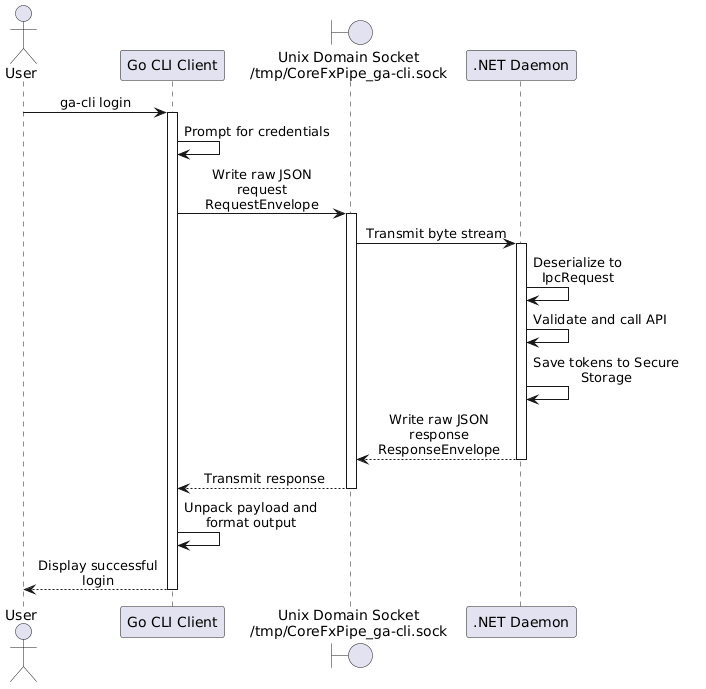
\includegraphics[width=0.8\textwidth]{images/ipc-sequence.png}
    \caption{Sekvenční diagram IPC komunikace při přihlášení.}
    \label{fig:ipcsequence}
\end{figure}

\subsection{Příklady zpráv}
Struktura požadavku obsahuje název příkazu (\texttt{command}), samotná data (\texttt{payload}) a kontext požadavku (\texttt{context}), který nese informace o volajícím uživateli.

Příklad požadavku na přihlášení (\texttt{login}):

\begin{minipage}{\linewidth}
\begin{lstlisting}[language={}]
{
  "command": "login",
  "payload": {
    "TeamName": "mojefirma",
    "UserName": "jan.novak@mojefirma.cz",
    "Password": "moje_tajne_heslo"
  },
  "context": {
    "LinuxId": "1000",
    "IsRoot": false
  }
}
\end{lstlisting}
\end{minipage}

Služba na tento požadavek odpovídá strukturovanou zprávou, která indikuje úspěch či selhání a vrací příslušná data nebo chybové hlášení.

Příklad úspěšné odpovědi:

\begin{minipage}{\linewidth}
\begin{lstlisting}[language={}]
{
  "success": true,
  "data": {
    "IsLoggedIn": true
  }
}
\end{lstlisting}
\end{minipage}

Příklad odpovědi při chybě (neplatné údaje):

\begin{minipage}{\linewidth}
\begin{lstlisting}[language={}]
{
  "success": false,
  "data": null,
  "error": "Invalid credentials"
}
\end{lstlisting}
\end{minipage}

\section{Návrh uživatelského rozhraní (CLI)}
% Zde:
% - Strom příkazů (ga login, ga connect, ga status).
% - Návrh interaktivního režimu (TUI) vs. skriptovacího režimu (flags).
% - Jak budou vypadat výstupy (barvičky pro lidi, JSON pro stroje).

\section{Bezpečnostní model}
% Zde:
% - Ukládání tokenů (kde budou fyzicky na disku).
% - Oprávnění k socketu (kdo smí poslat příkaz službě).
% - Zabezpečení proti neoprávněné manipulaci.

\section{Datový model a konfigurace}
% Zde:
% - Kde bude konfigurace (/etc/goodaccess vs ~/.config/goodaccess).
% - Co všechno se musí ukládat (aliasy bran, poslední připojení).


% Implementace
\chapter{Implementace}
\label{chap:implementace}

V této kapitole je detailně rozebrán samotný proces implementace navrženého řešení. Pozornost je věnována struktuře celého projektu a následně specifickým technickým výzvám spojeným s vývojem klientské aplikace v jazyce Go a úpravám systémové služby na platformě .NET.

\section{Struktura projektu a vývojové prostředí}
Jelikož se výsledný produkt skládá z několika oddělených, avšak spolupracujících částí, bylo zásadní správně navrhnout strukturu repozitáře. Repozitář je koncipován jako monorepo, které zastřešuje zdrojové kódy jak pro klientskou část (frontend), tak pro vrstvu systémové služby (backend). Tento přístup zjednodušuje správu závislostí a verzování.

Hlavní rozdělení repozitáře je následující:
\begin{itemize}
    \item \texttt{cli/} -- Obsahuje zdrojové kódy klientské aplikace napsané v jazyce Go. Kód je strukturován s ohledem na oddělení uživatelského rozhraní od komunikační logiky (adresáře \texttt{cmd/} a \texttt{internal/}).
    \item \texttt{services/} -- Zahrnuje .NET projekty představující systémovou službu, která běží na pozadí.
    \begin{itemize}
        \item \texttt{CLIService/} -- Nově vytvořený modul určený primárně pro obsluhu IPC komunikace s CLI klientem a řízení jeho požadavků.
        \item \texttt{GoodAccessService/} -- Původní jádro služby obstarávající infrastrukturu a samotné sestavování tunelů (např. OpenVPN, WireGuard).
    \end{itemize}
    \item \texttt{GoodAccess.Shared/} -- Sdílené doménové modely, rozhraní a utility využívané napříč různými .NET službami.
\end{itemize}

Architektura je tak striktně rozdělena na hloupého klienta (Go), který se stará pouze o prezentaci dat uživateli, a chytrou službu (.NET), kde probíhá veškerá složitá byznys logika.

\section{Implementace systémové služby (.NET)}
Aby bylo možné efektivně zpracovávat požadavky přicházející od CLI klienta, bylo nutné infrastrukturu na straně služby patřičně rozšířit. Vývoj probíhal iterativně počínaje zajištěním bezpečného úložiště a zprovozněním lokálního komunikačního kanálu.

\subsection{Meziprocesní komunikace (IPC)}
Základním kamenem architektury je nově vytvořený modul \texttt{CLIService}. Tento modul slouží jako most mezi uživatelskými vstupy a jádrem služby. Komunikace probíhá přes Unix Domain Sockets (UDS), což je na platformě Linux standardní a vysoce výkonný způsob výměny dat mezi lokálními procesy.

Služba vytvoří pojmenovanou rouru (named pipe), na které asynchronně naslouchá příchozím spojením od klienta. Požadavky jsou zasílány a vraceny ve formátu JSON, což usnadňuje deserializaci dat na obou stranách.

\begin{figure}[ht]
\begin{lstlisting}
// Ukázka inicializace IPC serveru pomocí NamedPipeServerStream pro Linux
var pipeServer = new NamedPipeServerStream(
    pipeName: "CoreFxPipe_ga-cli.sock",
    direction: PipeDirection.InOut,
    maxNumberOfServerInstances: 1,
    transmissionMode: PipeTransmissionMode.Byte,
    options: PipeOptions.Asynchronous);

await pipeServer.WaitForConnectionAsync(cancellationToken);
// Zpracování příchozích dat ze socketu...
\end{lstlisting}
\caption{Inicializace Unix Domain Socketu na straně .NET služby}
\label{fig:ipc_init}
\end{figure}

\subsection{Bezpečné úložiště (Secure Storage)}
Aplikace potřebuje uchovávat citlivá data jako jsou autentizační tokeny a privátní klíče. Původní implementace pro grafické rozhraní ukládala některá data do prostoru uživatele. Jelikož CLI je navrženo s možností trvalého spojení běžícího čistě na úrovni systému, muselo být úložiště přesunuto do bezpečného systémového adresáře.

Byla vytvořena třída reprezentující \textit{Secure Storage}. Fyzické uložení dat využívá soubory zabezpečené restriktivními přístupovými právy (\texttt{chmod 700}), čímž je zaručeno, že k souborům má přístup pouze vlastník procesu (v tomto případě uživatel \texttt{root}, pod kterým služba běží). Samotná data uvnitř souborů jsou navíc šifrována pomocí \texttt{DataProtection API}.

\subsection{Zpracování příkazů (CliMessenger)}
Za samotné odbavování příchozích zpráv zodpovídá komponenta \texttt{CliMessenger}. Každý požadavek ve formátu JSON obsahuje specifikaci příkazu (např. \texttt{login}, \texttt{connect}) a příslušné argumenty. \texttt{CliMessenger} tyto požadavky směruje na specifické služby v rámci .NET backendu.

V raných fázích vývoje, kdy ještě nebyla zcela implementována veškerá produkční logika a klientská aplikace se teprve formovala, vracela metoda \texttt{CliMessenger} provizorní pevně daná data (tzv. hardcoded odpovědi). Tento přístup umožnil paralelní vývoj -- UI se mohlo designovat a testovat proti konzistentnímu API bez čekání na dokončení komplexní aplikační logiky. Postupem času byly tyto provizorní odpovědi nahrazovány reálným napojením na síťové a autentizační subsystémy.

\section{Klientská aplikace a příkazy (Go)}
Na straně klienta bylo zvoleno využití jazyka Go, a to především pro jeho vynikající vlastnosti při vývoji CLI aplikací a schopnost kompilace do jediné statické binárky nezávislé na externích knihovnách na koncovém systému. 

\subsection{Struktura příkazů (Cobra)}
Základní aplikační kostra byla postavena na populárním frameworku Cobra. Tento nástroj umožňuje velmi snadno deklarovat stromovou strukturu příkazů, definovat argumenty (tzv. flags) a automaticky generovat nápovědu pro uživatele.

Hlavní příkaz \texttt{ga-cli} byl inicializován jako kořenový uzel (Root Command), ke kterému byly postupně přidávány dílčí příkazy odpovídající požadovaným akcím (login, setup, connect a další). Architektura frameworku Cobra navíc vybízí k přehlednému uspořádání kódu, kdy má každý příkaz svůj vlastní soubor v adresáři \texttt{cmd/}.

\begin{figure}[ht]
\begin{lstlisting}
// Ukázka inicializace kořenového příkazu
var rootCmd = &cobra.Command{
	Use:   "ga-cli",
	Short: "GoodAccess CLI klient",
	Long:  "Rozhraní příkazové řádky pro správu GoodAccess VPN na Linuxu.",
}

func init() {
	rootCmd.AddCommand(loginCmd)
	rootCmd.AddCommand(connectCmd)
	rootCmd.AddCommand(statusCmd)
	// Registrace dalších příkazů...
}
\end{lstlisting}
\caption{Definice struktury příkazů pomocí frameworku Cobra}
\label{fig:cobra_init}
\end{figure}

\subsection{Implementace příkazů a stavový report}
Jednotlivé příkazy byly do aplikace implementovány iterativním způsobem v logickém pořadí:
\begin{enumerate}
    \item \textbf{login / logout:} První krok zajišťující ověření uživatele a zisk patřičných tokenů k další komunikaci.
    \item \textbf{setup:} Konfigurace připojení – výběr vhodné brány (gateway) ze seznamu, nastavení požadovaného protokolu a definice parametru persistentní konektivity.
    \item \textbf{connect / disconnect:} Finální inicializace samotného šifrovaného tunelu, což původně zahrnovalo primárně integraci s \texttt{ProtoService} a stávajícím OpenVPN rozhraním.
\end{enumerate}

Během celého procesu implementace výše zmíněných příkazů se ukázal jako kritický podpůrný prvek příkaz \textbf{status}. Tento příkaz byl průběžně doplňován a využíván k rychlé diagnostice stavu. Fakticky fungoval jako bezpečný nástroj pro čtení dat ze \textit{Secure Storage}, který prokazoval, zda předchozí operace (např. uložení tokenu po loginu či modifikace preferované brány po setupu) proběhly úspěšně. V pozdějších fázích projektu umožňoval navíc zobrazení aktivní chybové hlášky nebo logu připojení z backendu v reálném čase.

\section{Pokročilé funkce a technické výzvy}
Během integrace stěžejních funkčních celků do architektury se objevilo několik netriviálních technických výzev, které vyžadovaly hlubší analýzu a návrh specializovaných řešení.

\subsection{Správa VPN spojení (OpenVPN)}
Samotné vytvoření šifrovaného tunelu skrze protokol OpenVPN těží z již existující architektury modulu \texttt{ProtoService}, který je nasazen na ostatních platformách. Pro potřeby CLI klienta tak stačilo mapovat požadavky z UDS rozhraní do podoby interních struktur sítě a volat sdílenou aplikační logiku. Modul automaticky vygeneruje odpovídající konfiguraci, sestaví spojení a na pozadí monitoruje stabilitu relace.

\subsection{Persistentní relace a vícero uživatelů}
Jednou z definovaných funkčností byla možnost navázání persistentního (trvalého) spojení, kdy VPN zůstává aktivní i po odhlášení aktuálního systémového uživatele nebo po restartu zařízení.
Tento požadavek s sebou přinesl zásadní problém týkající se izolace více Linuxových uživatelů.

Jelikož je sestavené VPN spojení systémového charakteru (routování přes rozhraní tunelu ovlivňuje globální směrovací tabulky stroje), mohlo by dojít k situaci, kdy jeden uživatel sestaví persistentní spojení a jiný uživatel po přihlášení nemá oprávnění jej modifikovat či ukončit, přestože je jeho síťový provoz rovněž šifrován.
Z toho důvodu bylo nutné obohatit komunikační protokol IPC o explicitní předávání systémového kontextu a identifikaci uživatele, který požadavek vznáší. Pokud je aktivní persistentní tunel spuštěný jiným uživatelem a nejedná se o autorizovanou operaci, je akce zamítnuta na úrovni služby. Administrátor pak musí relaci manuálně ukončit přes příkaz vyžadující superuživatelská práva, např. voláním \texttt{sudo ga-cli disconnect}.

\subsection{Implementace protokolu WireGuard}
Moderní protokol WireGuard představoval v kontextu architektury významnou výzvu, jelikož práce zahrnovala implementaci samotného agenta (sestavování sítě) cíleně pouze pro prostředí Linux s využitím statických konfigurací.
Na rozdíl od uceleného řízení (životní cyklus přes operační systém, dynamické doporučování gateway, automatické znovupřipojení), které přesahuje rámec této bakalářské práce a je paralelně vyvíjeno ostatními členy týmu na různých platformách, se tato konkrétní implementace zaměřuje primárně na fundamentální logiku navázání komunikace přes nativní systémové nástroje (ip link, wg). Tyto operace jsou vloženy do kontextu služeb \texttt{ProtoService} a tvoří základ budoucí robustní síťové logiky.

\subsection{Vylepšení uživatelské přívětivosti (UX)}
S cílem maximalizovat komfort koncových uživatelů při interakci v terminálu byl klient postupně doplňován o podpůrné funkce a takzvané přepínače (flags).
Příkladem je plná podpora pro strojově čitelné formátování výstupů prostřednictvím flagu \texttt{--json}, jenž zajišťuje, že aplikace nebude vracet interaktivní textové uživatelské rozhraní, ale naopak striktně strukturovaný JSON výstup. Tato funkce je naprosto nezbytná pro možnou integraci CLI do DevOps pipelinek a automatizačních skriptů, kde je vyžadováno bezobslužné řízení celého procesu připojení. Další UX optimalizace zahrnovaly vylepšení asynchronního logování stavu a přehlednější zpracování konfiguračních interakcí.


% Testování
\chapter{Testování a validace}
\label{chap:testovani}

Ověření funkčnosti a stability aplikace probíhalo v souladu s metodikou Extrémního programování průběžně během vývoje.

\section{Metodika testování}
\label{sec:metodika_testovani}

V souladu s principy agilního vývoje, zejména metodiky Extrémního programování (XP), bylo testování integrální součástí celého vývojového cyklu, nikoliv až jeho závěrečnou fází. Uplatňován byl přístup TDD (Test-Driven Development), kdy byly pro klíčové logické celky psány testy ještě před samotnou implementací. Tento postup nejenže zajistil vysoké pokrytí kódu, ale zároveň sloužil jako živá specifikace chování jednotlivých komponent \cite{beck_xp}.

Strategie testování byla založena na osvědčeném modelu testovací pyramidy, jak jej definoval Mike Cohn. Cílem bylo maximalizovat počet rychlých a levných jednotkových testů, které poskytují okamžitou zpětnou vazbu, a minimalizovat množství pomalých a křehkých end-to-end testů \cite{cohn_succeeding}.

\begin{itemize}
    \item \textbf{Jednotkové testy (Unit Tests):} Tvoří základnu pyramidy a ověřují funkčnost izolovaných komponent (funkcí, tříd) bez závislosti na externích systémech, jako je síťová komunikace nebo souborový systém.
    \item \textbf{Integrační testy (Integration Tests):} Testují spolupráci mezi jednotlivými moduly, například správnost komunikace mezi CLI klientem a systémovou službou přes IPC rozhraní.
    \item \textbf{End-to-End (E2E) testy:} Manuálně prováděné scénáře simulující kompletní uživatelskou cestu -- od spuštění příkazu v terminálu, přes sestavení VPN tunelu až po ověření síťové konektivity.
\end{itemize}

\section{Jednotkové testy a mockování}
\label{sec:unit_testing}

Největší důraz byl kladen na jednotkové testy, které umožňují rychlou a spolehlivou verifikaci aplikační logiky.

\subsection{Testování klienta v Go}
Pro testování CLI klienta napsaného v jazyce Go byl využit standardní vestavěný balíček \texttt{testing} v kombinaci s populární knihovnou \texttt{testify}, která poskytuje bohatší sadu nástrojů pro aserce (\texttt{assert}) a především pro mockování závislostí (\texttt{mock}).

Klíčovou technikou bylo mockování (vytváření atrap) pro rozhraní meziprocesové komunikace (IPC). Jelikož frontendová aplikace v Go komunikuje se backendovou službou v .NET přes Unix Domain Socket, bylo pro účely testování nezbytné tuto závislost odstranit. Tímto způsobem bylo možné testovat logiku a vzhled textového uživatelského rozhraní (TUI) zcela izolovaně, bez nutnosti mít spuštěnou a nakonfigurovanou systémovou službu.

Byl vytvořen mock klient \texttt{MockClient}, který implementuje stejné rozhraní jako reálný IPC klient. Pomocí knihovny \texttt{testify/mock} bylo možné předdefinovat očekávané chování -- tedy jakou odpověď má mock vrátit, když je zavolána jeho metoda \texttt{Send} s určitými parametry.

\lstinputlisting[language=Go, caption={Ukázka mock klienta pro IPC komunikaci}, label={lst:mock_client}]{../doc/code/mock_client.go}

Tento \texttt{MockClient} byl následně v testovacích scénářích (např. v souboru \texttt{setup\_test.go}) injektován do komponenty TUI namísto reálného klienta. Test tak mohl snadno simulovat různé scénáře, jako je úspěšné přihlášení, chyba spojení nebo příjem dat ze služby, a ověřit, že se uživatelské rozhraní chová dle očekávání.

\subsection{Testování služby v .NET}
Na straně systémové služby v .NET byly jednotkové testy navrženy s využitím frameworku xUnit. Ačkoliv nebyly plně implementovány v rámci této práce, jejich návrh počítal s testováním jednotlivých tříd v izolaci. Příkladem může být testování třídy \texttt{CliStorage}, která zodpovídá za bezpečné ukládání dat.

Příklad fiktivních testovacích scénářů pro třídu \texttt{CliStorage}:
\begin{itemize}
    \item \texttt{SavePreferences\_ShouldStoreCorrectData()}: Test ověří, že po zavolání metody \texttt{SavePreferences} je do souboru zapsán správně naformátovaný a zašifrovaný JSON objekt.
    \item \texttt{GetRefreshToken\_ShouldThrowOnMissingToken()}: Test zajistí, že pokud se metoda pokusí přečíst neexistující token, je vyhozena očekávaná výjimka.
    \item \texttt{SetRefreshToken\_ShouldUpdateSession()}: Ověří, že zavolání metody pro nastavení nového obnovovacího tokenu správně aktualizuje data v úložišti.
\end{itemize}

Tento přístup, založený na striktním oddělení závislostí a jejich mockování, je základním předpokladem pro udržitelný a spolehlivý vývoj komplexních systémových nástrojů.

\section{Integrační a systémové testy}
% Zde:
% - Testování komunikace Client <-> Service.
% - Ověření, že se VPN skutečně připojí (ping, ip route).

\section{Testování na různých distribucích}
% Zde:
% - Tabulka kompatibility (Debian, Fedora, Ubuntu).
% - Zkušenosti z "reálného provozu" (pokud jsi to někomu dal zkusit).


% Závěr (musí obsahovat \addchap{Závěr})
\addchap{Závěr}
\label{chap:zaver}

Cílem této bakalářské práce byl návrh a implementace nativního CLI klienta GoodAccess pro OS Linux.

\section*{Shrnutí výsledků}
% Zde:
% - Stručně: Povedlo se to. Máme klienta, umí WireGuard, je bezpečný.
% - Porovnání se zadáním (všechny body splněny).

\section*{Diskuse a přínos}
% Zde:
% - V čem je toto řešení lepší než to, co tam bylo (nebo nebylo) předtím.
% - Jak to pomůže adminům (automatizace).

\section*{Možnosti budoucího rozvoje}
% Zde:
% - Co se nestihlo nebo nebylo v zadání.
% - Např. podpora pro Split Tunneling v TUI, notifikace na desktopu, podpora dalších dister (Arch).


% ============================================================================
% LITERATURA A PŘÍLOHY
% ============================================================================


\sloppy
\printbibliography[title=Seznam použitých zdrojů]

\appendix

\chapter{Externí přílohy\label{sec:ep}}

Externí přílohy této bakalářské práce jsou umístěny na veřejném úložišti GitHub na adrese:\\ \url{https://github.com/ValdemarPospisil/Bachelors}.

Vzhledem k tomu, že vývoj aplikace probíhal v rámci firemního prostředí společnosti GoodAccess, je samotný zdrojový kód aplikace soukromý a podléhá obchodnímu tajemství. Tento veřejný repozitář slouží jako doprovodný materiál k textu práce a obsahuje dokumentaci, vybrané ukázky kódu, schémata a specifikace testů, které dokumentují technickou náročnost a rozsah řešení.

Na úložišti jsou k dispozici tyto materiály:

\begin{itemize}
\item \textbf{Ukázky zdrojových kódů} – vybrané části implementace v jazycích Go (frontend) a C\# (backend).
\item \textbf{Specifikace testů} – BDD scénáře v jazyce Gherkin pro klíčové funkce systému.
\item \textbf{Schémata a diagramy} – architektura systému, sekvenční diagramy IPC a roadmapa projektu v původním rozlišení.
\item \textbf{Screenshoty} – snímky obrazovky zachycující reálný provoz aplikace, interaktivní průvodce nastavením a chybové stavy.
\item \textbf{Dokumentace} – doprovodné technické texty a zdrojové soubory bakalářské práce.
\end{itemize}

V následující tabulce je uvedena základní struktura úložiště:

\begin{longtable}{ll}
\hline
\textbf{Složka / Soubor} & \textbf{Popis} \\
\hline
\texttt{README.md} & Hlavní přehled projektu s Mermaid diagramy a náhledy. \\
\texttt{thesis/thesis.pdf} & Vygenerovaný PDF výstup bakalářské práce. \\
\texttt{thesis/} & Zdrojové texty bakalářské práce v systému \LaTeX{}. \\
\texttt{thesis/images/} & Kompletní sada obrázků a screenshotů použitých v práci. \\
\texttt{doc/code/} & Vybrané ukázky zdrojových kódů (frontend i backend). \\
\texttt{doc/specs/} & Akceptační testy a specifikace v jazyce Gherkin. \\
\texttt{doc/diagrams/} & Schémata architektury a roadmapa projektu. \\
\texttt{doc/screenshots/} & Doplňkové snímky obrazovky z reálného provozu aplikace. \\
\texttt{presentations/} & Prezentace práce vytvořená v rámci semináře SKKI1. \\
\hline
\end{longtable}

\end{document}
